\documentclass{article}
\usepackage{amsmath}
\usepackage{amssymb}
\usepackage{enumitem}
\usepackage{cancel}

\usepackage{xcolor}
\usepackage[colorlinks=true,bookmarks=false,linkcolor=black,urlcolor=blue,citecolor=black]{hyperref}
\usepackage[top=1in,bottom=1in,left=1in,right=1in]{geometry}

\usepackage{fancyhdr}
\let\temp\rmdefault
\usepackage{mathpazo}
\let\rmdefault\temp

\usepackage{pgfplots}
\pgfplotsset{compat=1.8}

\usetikzlibrary{shapes,arrows,positioning,calc}
\definecolor{roseRed}{HTML}{e20047}
\definecolor{coolGray}{HTML}{474747} % Neutral gray to contrast roseRed
\definecolor{mocha}{HTML}{a47864}
\definecolor{sage}{HTML}{8a9a5b}
\definecolor{dustyblue}{HTML}{6e8ca0}
\definecolor{terracotta}{HTML}{c87f5b}
\definecolor{lavender}{HTML}{9d8bb0}
\definecolor{darkmocha}{HTML}{7a5a4b}
\definecolor{darksage}{HTML}{667244}
\definecolor{darkdustyblue}{HTML}{526878}
\definecolor{darkterracotta}{HTML}{9e6347}
\definecolor{darklavender}{HTML}{766688}
\definecolor{winery}{HTML}{7e212a}

\definecolor{lightmocha}{HTML}{c2a190}
\definecolor{lightmocha1}{HTML}{d1b09c}
\definecolor{lightmocha2}{HTML}{e2c4b0}
\definecolor{lightmocha3}{HTML}{f0d9c7}

\definecolor{androidBlue}{HTML}{8AB4F8}
\definecolor{androidBlueLight}{HTML}{E8F0FE}
\definecolor{androidGreen}{HTML}{81C995}
\definecolor{androidGreenLight}{HTML}{E6F4EA}

% Red variants - based on Android's "error" and warning colors
\definecolor{androidRed}{HTML}{F28B82}
\definecolor{androidRedLight}{HTML}{FADAD7}

% Yellow variants - based on Android's accent/warning colors
\definecolor{androidYellow}{HTML}{FDD663}
\definecolor{androidYellowLight}{HTML}{FEF7E0}

% Purple variants - based on Android's system UI accents
\definecolor{androidPurple}{HTML}{D7AEFB}
\definecolor{androidPurpleLight}{HTML}{F4EAFC}

% Orange variants - based on Android's notification colors
\definecolor{androidOrange}{HTML}{FCAD70}
\definecolor{androidOrangeLight}{HTML}{FEEADC}

% Teal variants - based on Android's Material You palette
\definecolor{androidTeal}{HTML}{78D9EC}
\definecolor{androidTealLight}{HTML}{E6F6F9}

% Gray variants - based on Android's neutral colors
\definecolor{androidGray}{HTML}{DADCE0}
\definecolor{androidGrayLight}{HTML}{F1F3F4}



\usepackage[many]{tcolorbox}

% Redefine \maketitle to include tcolorbox
\makeatletter
\renewcommand{\maketitle}{%
    \begin{center}
        \begin{tcolorbox}[
            enhanced,
            colback=white,
            colframe=red!70!black,
            arc=0mm,
            title={\textcolor{white}{\bfseries CPE 381 \@title}},
            coltitle=white,
            fonttitle=\bfseries\large,
            attach boxed title to top left={xshift=10pt, yshift=-\tcboxedtitleheight/2},
            boxed title style={
            sharp corners,
            colback=red!70!black,
            frame hidden,
            boxrule=0pt,
            left=10pt, right=10pt,
            top=3pt, bottom=3pt
            }
        ]
        \large
        \vspace{10pt}
        \noindent Instructor: Rahul Bhadani 
        

            \end{tcolorbox}
    \end{center}
}
\makeatother

\usepackage{biolinum} % included with the {Libertine} font package
\renewcommand{\familydefault}{\sfdefault}



\newcommand{\hw}{Problems in Laplace Transform}
\newcommand{\duedate}{}
\newcommand{\hwturnin}{cw11}

% Add showanswer toggle (set to "yes" for solutions, anything else for student version)
\usepackage{ifthen}
\newcommand{\showanswer}{yes}

\newenvironment{multiequation}[1][]{%
    \begin{equation}%
    \begin{aligned}%
        \ifx#1\@empty\else\label{#1}\fi%
}{%
    \end{aligned}%
\end{equation}% 
}
\pagestyle{fancy}

\lhead{\footnotesize{CPE 381}, \footnotesize{The University of Alabama in Huntsville}}
\chead{}
\rhead{\footnotesize{\emph{\hw}}}
\lfoot{\footnotesize{Rahul Bhadani}}
\cfoot{\footnotesize{\thepage}}
\rfoot{\footnotesize{\textit{Last Revised:~\today}}}
\renewcommand{\headrulewidth}{0.1pt}
\renewcommand{\footrulewidth}{0.1pt}
\newcommand{\minipagewidth}{0.8\columnwidth}

\renewcommand{\thefootnote}{\fnsymbol{footnote}}


\renewcommand{\headrulewidth}{0.1pt}
\renewcommand{\footrulewidth}{0.1pt}

\renewcommand{\thefootnote}{\fnsymbol{footnote}}
\begin{document}

\title{\textsc{\hw}}
\author{Instructor: \instructorname}
\date{Due: \duedate\\ 100 points}

\maketitle


\section{Second-Order System Analysis}
A system is described by the differential equation:
\[ \frac{d^2y(t)}{dt^2} + 5\frac{dy(t)}{dt} + 6y(t) = \frac{dx(t)}{dt} + 2x(t) \]
\begin{enumerate}[label=(\alph*)]
    \item Find the transfer function $H(s) = \frac{Y(s)}{X(s)}$
    \item Determine all poles and zeros of the system
    \item Find the impulse response $h(t)$ for the causal system
    \item Analyze the stability of the causal system
    \item Find the step response of the system
\end{enumerate}

\textbf{Solution:}
\begin{enumerate}[label=(\alph*)]
    \item Taking Laplace transform of both sides (assuming zero initial conditions):
    \begin{align*}
        s^2Y(s) + 5sY(s) + 6Y(s) &= sX(s) + 2X(s) \\
        (s^2 + 5s + 6)Y(s) &= (s + 2)X(s) \\
        H(s) &= \frac{Y(s)}{X(s)} = \frac{s + 2}{s^2 + 5s + 6}
    \end{align*}
    
    \item Factoring numerator and denominator:
    \begin{align*}
        H(s) &= \frac{s + 2}{(s + 2)(s + 3)} \\
        \text{Zero: } & s = -2 \\
        \text{Poles: } & s = -2, -3 \quad \text{(Note: pole-zero cancellation at } s = -2)
    \end{align*}
    
    \item After pole-zero cancellation:
    \begin{align*}
        H(s) &= \frac{1}{s + 3}, \quad \text{Region of Convergence, ROC: } \text{Re}\{s\} > -3 \\
        h(t) &= e^{-3t}u(t)
    \end{align*}
    
    \item The system is stable because the only pole is at $s = -3$ (in Left Hand Plane (LHP)) and the ROC includes the $j\Omega$-axis.
    
    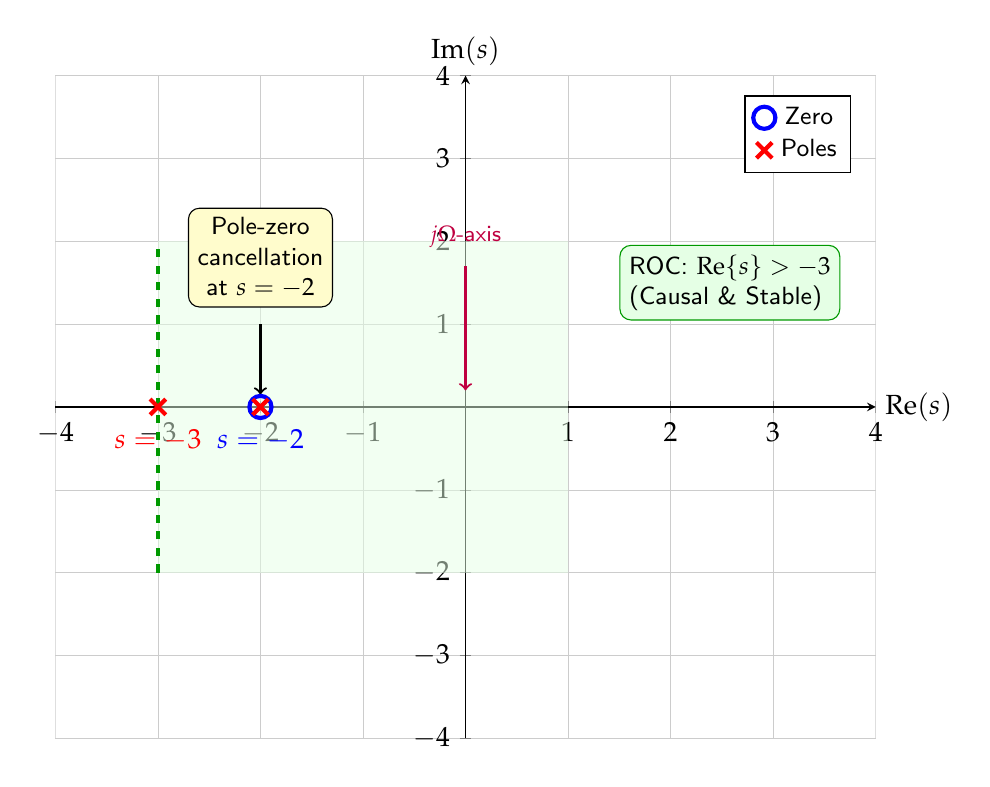
\begin{tikzpicture}
    \begin{axis}[
        width=12cm,
        height=10cm,
        axis lines=middle,
        xlabel={$\mathrm{Re}(s)$},
        ylabel={$\mathrm{Im}(s)$},
        xlabel style={anchor=west},
        ylabel style={anchor=south},
        xmin=-4, xmax=4,
        ymin=-4, ymax=4,
        xtick={-4,-3,-2,-1,0,1, 2, 3, 4},
        ytick={-4, -3, -2,-1,0,1,2, 3, 4},
        grid=both,
        grid style={line width=.1pt, draw=gray!20},
        major grid style={line width=.2pt,draw=gray!40},
        axis equal image=false,
        legend pos=north east,
        legend style={draw=black, fill=white, font=\small}
    ]
    
    % Zero at s = -2 (circle)
    \addplot[only marks, mark=o, mark size=4pt, line width=1.5pt, color=blue] 
        coordinates {(-2,0)};
    \addlegendentry{Zero}
    
    % Pole at s = -2 (crosses) - cancels with zero
    \addplot[only marks, mark=x, mark size=4pt, line width=1.5pt, color=red] 
        coordinates {(-2,0)};
    \addlegendentry{Poles}
    
    % Pole at s = -3 (cross)
    \addplot[only marks, mark=x, mark size=4pt, line width=1.5pt, color=red] 
        coordinates {(-3,0)};
    
    % Draw ROC (Region of Convergence) as shaded region
    \fill[green!10, opacity=0.5] (axis cs:-3,2) rectangle (axis cs:1,-2);
    
    % Draw ROC boundary line
    \addplot[dashed, very thick, color=green!60!black, domain=-2:2] ({-3}, x);
    
    % Annotations for poles
    \node[anchor=north, color=red] at (axis cs:-3,-0.15) {$s=-3$};
    \node[anchor=north, color=blue] at (axis cs:-2,-0.15) {$s=-2$};
    
    % Pole-zero cancellation annotation
    \node[anchor=south, font=\small, align=center, fill=yellow!20, draw=black, rounded corners] 
        at (axis cs:-2,1.2) {Pole-zero\\cancellation\\at $s=-2$};
    \draw[->, thick] (axis cs:-2,1.0) -- (axis cs:-2,0.15);
    
    % ROC annotation
    \node[anchor=west, font=\small, align=left, fill=green!10, draw=green!60!black, rounded corners] 
        at (axis cs:1.5,1.5) {ROC: $\mathrm{Re}\{s\} > -3$\\(Causal \& Stable)};
    
    % jΩ axis indicator
    \node[anchor=south, font=\footnotesize, color=purple] at (axis cs:0,1.8) {$j\Omega$-axis};
    \draw[->, thick, color=purple] (axis cs:0,1.7) -- (axis cs:0,0.2);
    
    \end{axis}
\end{tikzpicture}

    \item Step response:
    \begin{align*}
        Y(s) &= H(s)X(s) = \frac{1}{s + 3} \cdot \frac{1}{s} = \frac{1}{s(s + 3)} \\
        &= \frac{A}{s} + \frac{B}{s + 3} \\
    \end{align*}
    
    Doing cross multiplication for RHS
    
    \begin{align*}
    Y(s) & = \frac{As + 3A + Bs}{s(s+3)}
    \end{align*}
    Equation coefficients of $s$ both sides
    
    \begin{align*}
    A + B & = 0\\
    3A & = 1 \Rightarrow A = \frac{1}{3}, \quad B = -A =-\frac{1}{3}
    \end{align*}
    
    Hence, 
    
    \begin{align*}
    Y(s) = \frac{1}{3s} - \frac{1}{3}\frac{1}{s+3}
    \end{align*}
    
    Using Laplace transform table, 
    
    \begin{align*}
    y(t) = \frac{1}{3}u(t) - \frac{1}{3}e^{-3t}u(t)
    \end{align*}
\end{enumerate}

\section{System Stability Analysis}
Given the transfer function:
\[ H(s) = \frac{s^2 + 4s + 13}{(s + 1)(s^2 + 2s + 5)} \]
\begin{enumerate}[label=(\alph*)]
    \item Find all poles and zeros
    \item Determine the possible ROCs and corresponding system properties (causal/anti-causal, stable/unstable)
    \item For the causal case, find the impulse response
    \item Check if the system is BIBO stable when causal
\end{enumerate}

\textbf{Solution:}
\begin{enumerate}[label=(\alph*)]
    \item Finding poles and zeros:
    \begin{align*}
        \text{Zeros: } & s^2 + 4s + 13 = 0 \Rightarrow s = -2 \pm 3j \\
        \text{Poles: } & s = -1, \quad s^2 + 2s + 5 = 0 \Rightarrow s = -1 \pm 2j
    \end{align*}
    
    \item Possible ROCs:
    \begin{itemize}
        \item $\text{Re}\{s\} > -1$: Causal, stable (ROC  includes $j\Omega$-axis)
        \item $-1 < \text{Re}\{s\} < -1$: Not possible (poles at same real part)
        \item $\text{Re}\{s\} < -1$: Anti-causal, unstable
    \end{itemize}
    
    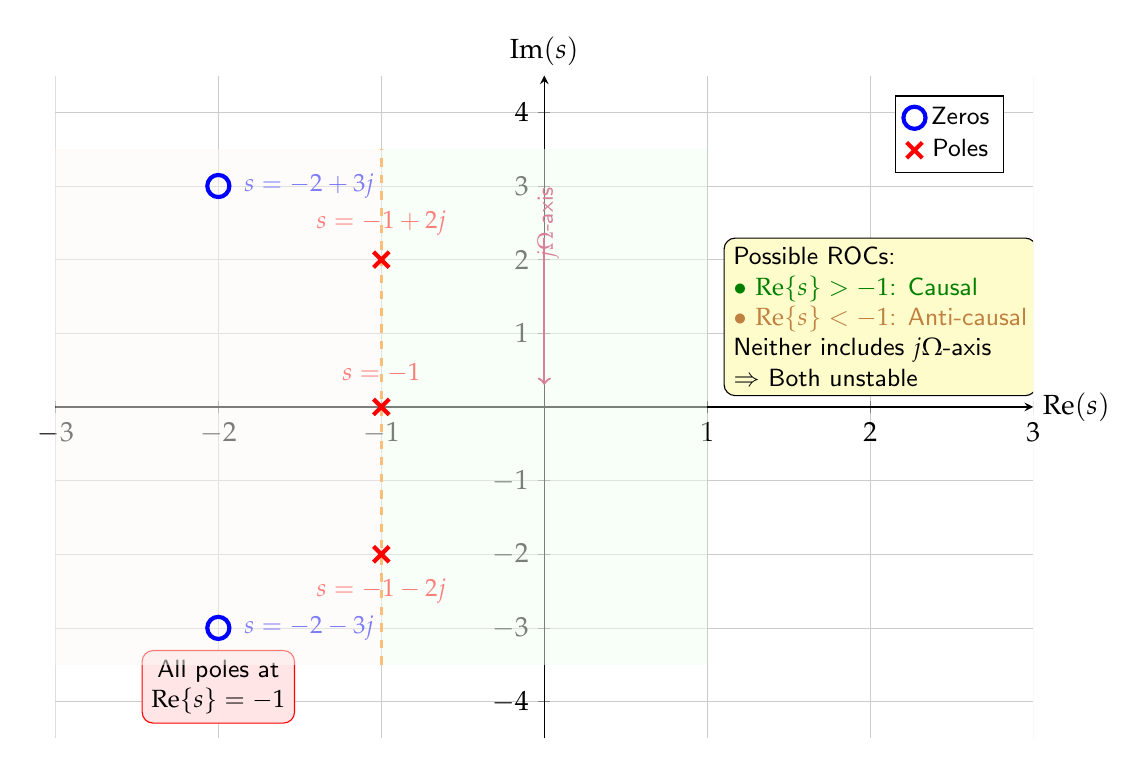
\begin{tikzpicture}
    \begin{axis}[
        width=14cm,
        height=10cm,
        axis lines=middle,
        xlabel={$\mathrm{Re}(s)$},
        ylabel={$\mathrm{Im}(s)$},
        xlabel style={anchor=west},
        ylabel style={anchor=south},
        xmin=-3, xmax=3,
        ymin=-4.5, ymax=4.5,
        xtick={-3,-2,-1,0,1, 2, 3},
        ytick={-4, -3,-2,-1,0,1,2,3, 4},
        grid=both,
        grid style={line width=.1pt, draw=gray!20},
        major grid style={line width=.2pt,draw=gray!40},
        axis equal image=false,
        legend pos=north east,
        legend style={draw=black, fill=white, font=\small}
    ]
    
    % Zeros (circles) - complex conjugate pair at s = -2 ± 3j
    \addplot[only marks, mark=o, mark size=4pt, line width=1.5pt, color=blue] 
        coordinates {(-2,3) (-2,-3)};
    \addlegendentry{Zeros}
    
    % Poles (crosses)
    % Pole at s = -1 (real axis)
    \addplot[only marks, mark=x, mark size=4pt, line width=1.5pt, color=red] 
        coordinates {(-1,0)};
    \addlegendentry{Poles}
    
    % Poles - complex conjugate pair at s = -1 ± 2j
    \addplot[only marks, mark=x, mark size=4pt, line width=1.5pt, color=red] 
        coordinates {(-1,2) (-1,-2)};
    
    % Vertical line at Re{s} = -1 showing all poles have same real part
    \addplot[dashed, very thick, color=orange, domain=-3.5:3.5] ({-1}, x);
    
    % Annotations for zeros
    \node[anchor=west, color=blue, font=\small] at (axis cs:-1.9,3) {$s=-2+3j$};
    \node[anchor=west, color=blue, font=\small] at (axis cs:-1.9,-3) {$s=-2-3j$};
    
    % Annotations for poles
    \node[anchor=south, color=red, font=\small] at (axis cs:-1,0.2) {$s=-1$};
    \node[anchor=south, color=red, font=\small] at (axis cs:-1,2.2) {$s=-1+2j$};
    \node[anchor=north, color=red, font=\small] at (axis cs:-1,-2.2) {$s=-1-2j$};
    
    % jΩ axis indicator
    \node[anchor=south, font=\footnotesize, color=purple, rotate=90] at (axis cs:0.15,2.5) {$j\Omega$-axis};
    \draw[->, thick, color=purple] (axis cs:0,2.3) -- (axis cs:0,0.3);
    
    % ROC annotations
    \node[anchor=north, font=\small, align=center, fill=red!10, draw=red, rounded corners] 
        at (axis cs:-2,-3.3) {All poles at\\$\mathrm{Re}\{s\} = -1$};
    
    \node[anchor=north west, font=\small, align=left, fill=yellow!20, draw=black, rounded corners] 
        at (axis cs:1.1,2.3) {Possible ROCs:\\
        \textcolor{green!50!black}{$\bullet$ $\mathrm{Re}\{s\} > -1$: Causal}\\
        \textcolor{brown}{$\bullet$ $\mathrm{Re}\{s\} < -1$: Anti-causal}\\
        Neither includes $j\Omega$-axis\\
        $\Rightarrow$ Both unstable};
    
    % Shade ROC regions lightly
    % Causal ROC: Re{s} > -1
    \fill[green!5, opacity=0.5] (axis cs:-1,3.5) rectangle (axis cs:1,-3.5);
    
    % Anti-causal ROC: Re{s} < -1
    \fill[brown!5, opacity=0.5] (axis cs:-3,3.5) rectangle (axis cs:-1,-3.5);
    
    \end{axis}
\end{tikzpicture}

    \item For causal case ($\text{Re}\{s\} > -1$):
    \begin{align*}
        H(s) &= \frac{s^2 + 4s + 13}{(s + 1)(s^2 + 2s + 5)} = \frac{A}{s + 1} + \frac{Bs + C}{s^2 + 2s + 5}
    \end{align*}
    Solving for coefficients:
   
   \begin{align*}
   H(s) & = \frac{As^2 + 2sA + 5A + Bs^2 + Cs + Bs + C}{(s + 1)(s^2 + 2s + 5)}\\
   A + B & = 1 \Rightarrow  B = 1 - A\\
   5A + C & = 13 \Rightarrow C = 13 - 5A\\
   2A + B + C  & = 4 \Rightarrow 2A  + 1 - A + 13 - 5A = 4\\
 \Rightarrow -4A & = -10 \Rightarrow A = 2.5\\
 B & = 1-2.5 = -1.5, \quad C = 13 - 5\times \frac{5}{2} = 13 - 12.5 = 0.5
   \end{align*}

    Therefore:
    \begin{align*}
        H(s) &= \frac{2.5}{s + 1} + \frac{-1.5s + 0.5}{s^2 + 2s + 5} \\
        &= \frac{2.5}{s + 1} - 1.5 \cdot \frac{s + 1}{(s + 1)^2 + 4} + 2 \cdot \frac{1}{(s + 1)^2 + 4} =  \frac{2.5}{s + 1} - 1.5 \cdot \frac{s + 1}{(s + 1)^2 + 2^2} +  \cdot \frac{2}{(s + 1)^2 + 2^2}
    \end{align*}
    Taking inverse Laplace transform using Tables:
    \[ h(t) = [2.5e^{-t} - 1.5e^{-t}\cos(2t) + e^{-t}\sin(2t)]u(t) \]
    
    \item The causal system is stable because the ROC ($\text{Re}\{s\} > -1$) includes the $j\Omega$-axis, and all poles are in left-half plane.
\end{enumerate}

\section{Mass-Spring-Damper System}
A mass-spring-damper system is described by:
\[ m\frac{d^2y(t)}{dt^2} + b\frac{dy(t)}{dt} + ky(t) = x(t) \]
where $m = 1$ kg, $b = 4$ Ns/m, $k = 13$ N/m, and $x(t)$ is the applied force.
\begin{enumerate}[label=(\alph*)]
    \item Find the transfer function
    \item Determine the poles and characterize the system response (overdamped, underdamped, or critically damped)
    \item Find the impulse response
    \item Find the response to a unit step input
\end{enumerate}

\textbf{Solution:}
\begin{enumerate}[label=(\alph*)]
    \item With given values:
    \begin{align*}
        \frac{d^2y(t)}{dt^2} + 4\frac{dy(t)}{dt} + 13y(t) &= x(t) \\
        s^2Y(s) + 4sY(s) + 13Y(s) &= X(s) \\
        H(s) &= \frac{Y(s)}{X(s)} = \frac{1}{s^2 + 4s + 13}
    \end{align*}
    
    \item Poles:
    \begin{align*}
        s^2 + 4s + 13 &= 0 \Rightarrow s = -2 \pm 3j
    \end{align*}
    Complex conjugate poles with negative real parts indicate an underdamped system.
    
    \item Impulse response:
    \begin{align*}
        H(s) &= \frac{1}{(s + 2)^2 + 9} = \frac{1}{3} \cdot \frac{3}{(s + 2)^2 + 3^2} \\
        h(t) &= \frac{1}{3}e^{-2t}\sin(3t)u(t)
    \end{align*}
    
    \item Step response:
    \begin{align*}
        Y(s) &= H(s)X(s) = \frac{1}{s(s^2 + 4s + 13)} \\
        &= \frac{A}{s} + \frac{Bs + C}{s^2 + 4s + 13}
    \end{align*}

\begin{align*}
 \frac{1}{s(s^2 + 4s + 13)}  & = \frac{As^2 + 4sA + 13A + Bs^2 + Cs}{s(s^2 + 4s + 13)}\\
 \Rightarrow 13A & = 1\Rightarrow A = \frac{1}{13}\\
 A + B & = 0 \Rightarrow B = -A = -\frac{1}{13}\\
 4A + C & = 0 \Rightarrow C = -4A = -\frac{4}{13}
\end{align*}

    Therefore:
    \begin{align*}
        Y(s) &= \frac{1}{13} \cdot \frac{1}{s} - \frac{1}{13} \cdot \frac{s + 4}{s^2 + 4s + 13} \\
        &= \frac{1}{13} \cdot \frac{1}{s} - \frac{1}{13} \cdot \frac{s + 2}{(s + 2)^2 + 9} - \frac{2}{39} \cdot \frac{3}{(s + 2)^2 + 9}
    \end{align*}
    Taking inverse Laplace transform:
    \[ y(t) = \frac{1}{13}[1 - e^{-2t}\cos(3t) - \frac{2}{3}e^{-2t}\sin(3t)]u(t) \]
\end{enumerate}

\section{RLC Circuit Analysis}
An RLC circuit has the transfer function:
\[ H(s) = \frac{V_{out}(s)}{V_{in}(s)} = \frac{s}{s^2 + 2s + 2} \]
\begin{enumerate}[label=(\alph*)]
    \item Find the differential equation relating $v_{out}(t)$ and $v_{in}(t)$
    \item Determine all poles and zeros
    \item Find the impulse response for the causal system
    \item Is the system stable? Justify your answer
    \item Find the frequency response $H(j\Omega)$
\end{enumerate}

\textbf{Solution:}
\begin{enumerate}[label=(\alph*)]
    \item From the transfer function:
    \begin{align*}
        H(s) &= \frac{V_{out}(s)}{V_{in}(s)} = \frac{s}{s^2 + 2s + 2} \\
        (s^2 + 2s + 2)V_{out}(s) &= sV_{in}(s)
    \end{align*}
    Taking inverse Laplace transform:
    \[ \frac{d^2v_{out}(t)}{dt^2} + 2\frac{dv_{out}(t)}{dt} + 2v_{out}(t) = \frac{dv_{in}(t)}{dt} \]
    
    \item Poles and zeros:
    \begin{align*}
        \text{Zero: } & s = 0 \\
        \text{Poles: } & s^2 + 2s + 2 = 0 \Rightarrow s = -1 \pm j
    \end{align*}
    
    \item Impulse response:
    \begin{align*}
        H(s) &= \frac{s}{(s + 1)^2 + 1} = \frac{s + 1}{(s + 1)^2 + 1} - \frac{1}{(s + 1)^2 + 1} \\
        h(t) &= [e^{-t}\cos(t) - e^{-t}\sin(t)]u(t)
    \end{align*}
    
    \item The system is stable because both poles are in the LHP ($s = -1 \pm j$) and the ROC for the causal system ($\text{Re}\{s\} > -1$) includes the $j\Omega$-axis.
    
    \item Frequency response:
    \begin{align*}
        H(j\Omega) &= H(s)\bigg|_{s = j\Omega} = \frac{j\Omega}{(j\Omega)^2 + 2j\Omega + 2} = \frac{j\Omega}{-\Omega^2 + 2j\Omega + 2}
    \end{align*}
\end{enumerate}

\section{Feedback System Analysis}
Consider a feedback system with forward path transfer function $G(s) = \frac{1}{s+2}$ and feedback path $H(s) = \frac{1}{s+1}$.
\begin{enumerate}[label=(\alph*)]
    \item Find the overall closed-loop transfer function
    \item Determine all poles and zeros of the closed-loop system
    \item Analyze the stability of the closed-loop system
    \item Compare the stability with the open-loop system
    \item Find the step response of the closed-loop system
\end{enumerate}

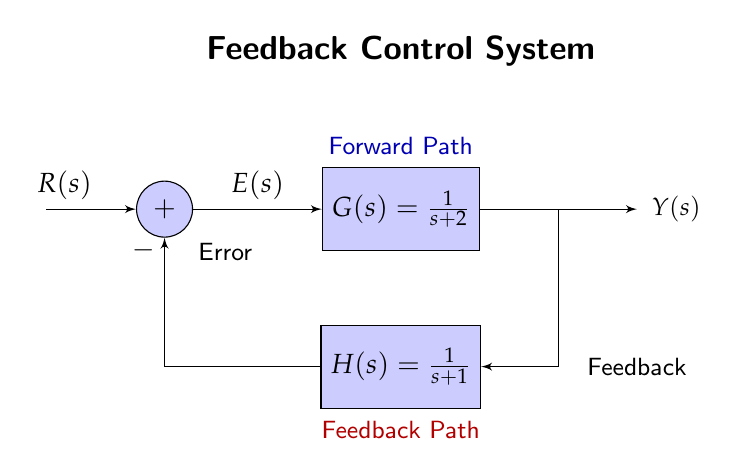
\begin{tikzpicture}[auto, node distance=2cm, >=latex']
    % Define block styles
    \tikzstyle{block} = [draw, fill=blue!20, rectangle, 
        minimum height=3em, minimum width=4em]
    \tikzstyle{sum} = [draw, fill=blue!20, circle, node distance=1.5cm]
    \tikzstyle{input} = [coordinate]
    \tikzstyle{output} = [coordinate]
    \tikzstyle{pinstyle} = [pin edge={to-,thin,black}]

    % Nodes
    \node [input, name=input] {};
    \node [sum, right of=input] (sum) {$+$};
    \node [block, right of=sum, node distance=3cm] (controller) {$G(s) = \frac{1}{s+2}$};
    \node [output, right of=controller, node distance=3cm] (output) {};
    \node [block, below of=controller, node distance=2cm] (feedback) {$H(s) = \frac{1}{s+1}$};
    
    % Connection nodes for better routing
    \coordinate[right of=controller, node distance=2cm] (measure);
    
    % Arrows and labels
    \draw [draw,->] (input) -- node[pos=0.2] {$R(s)$} (sum);
    \draw [->] (sum) -- node[pos=0.5, above] {$E(s)$} (controller);
    \draw [->] (controller) -- node [name=y, pos=0.5] {} (output);
    \draw [->] (measure) |- (feedback);
    \draw [->] (feedback) -| node[pos=0.95, left] {$-$} (sum);
      \node [right of=controller, node distance=3.5cm, font=\small] {$Y(s)$};
    
    
    % Labels on the feedback path
    \node [below right=0.05cm and 0.05cm of sum, font=\small] {Error};
    \node [right of=feedback, node distance=3.0cm, font=\small] {Feedback};
    
    % Title
    \node [above of=controller, node distance=2cm, font=\large\bfseries] {Feedback Control System};
    
    % Forward and Feedback path labels
    \node [above of=controller, node distance=0.8cm, font=\small, color=blue!70!black] {Forward Path};
    \node [below of=feedback, node distance=0.8cm, font=\small, color=red!70!black] {Feedback Path};
    
\end{tikzpicture}

\textbf{Solution:}
\begin{enumerate}[label=(\alph*)]
    \item Closed-loop transfer function:
    \begin{align*}
        T(s) &= \frac{G(s)}{1 + G(s)H(s)} = \frac{\frac{1}{s+2}}{1 + \frac{1}{(s+2)(s+1)}} \\
        &= \frac{\frac{1}{s+2}}{\frac{(s+2)(s+1) + 1}{(s+2)(s+1)}} = \frac{1}{s^2 + 3s + 3}
    \end{align*}
    
    \item Poles and zeros:
    \begin{align*}
        \text{Zeros: } & \text{None} \\
        \text{Poles: } & s^2 + 3s + 3 = 0 \Rightarrow s = -\frac{3}{2} \pm j\frac{\sqrt{3}}{2}
    \end{align*}
    
    \item The closed-loop system is stable because both poles have negative real parts ($-\frac{3}{2} \pm j\frac{\sqrt{3}}{2}$).
    
    \item Open-loop transfer function: $G(s)H(s) = \frac{1}{(s+2)(s+1)}$ has poles at $s = -1, -2$ (stable). Both open-loop and closed-loop are stable, but feedback changed the pole locations.
    
    \item Step response:
    \begin{align*}
        Y(s) &= T(s)X(s) = \frac{1}{s(s^2 + 3s + 3)} \\
        &= \frac{A}{s} + \frac{Bs + C}{s^2 + 3s + 3}
    \end{align*}
	
	\begin{align*}
		\frac{1}{s(s^2 + 3s + 3)} & = \frac{As^2 + 3As + 3A + Bs^2 + Cs}{s(s^2 + 3s + 3)}\\
		A & = \frac{1}{3}\\
		A + B & = 0 \Rightarrow B = -A = -\frac{1}{3}\\
		3A + C & = 0 \Rightarrow C = -3A = -1
	\end{align*}	    
    
    Therefore:
    \begin{align*}
        Y(s) &= \frac{1}{3} \cdot \frac{1}{s} - \frac{1}{3} \cdot \frac{s + 3}{s^2 + 3s + 3}
    \end{align*}
    Complete the square: $s^2 + 3s + 3 = (s + \frac{3}{2})^2 + (\frac{\sqrt{3}}{2})^2$
    \begin{align*}
        Y(s) &= \frac{1}{3} \cdot \frac{1}{s} - \frac{1}{3} \cdot \frac{s + \frac{3}{2}}{(s + \frac{3}{2})^2 + (\frac{\sqrt{3}}{2})^2} - \frac{1}{2\sqrt{3}} \cdot \frac{\frac{\sqrt{3}}{2}}{(s + \frac{3}{2})^2 + (\frac{\sqrt{3}}{2})^2}
    \end{align*}
    Taking inverse Laplace transform:
    \[ y(t) = \frac{1}{3}[1 - e^{-3t/2}\cos(\frac{\sqrt{3}}{2}t) - \frac{\sqrt{3}}{2}e^{-3t/2}\sin(\frac{\sqrt{3}}{2}t)]u(t) \]
\end{enumerate}

\section{Partial Fraction Expansion with Repeated Poles}
Given the transfer function:
\[ H(s) = \frac{s^2 + 3s + 3}{(s + 1)^3} \]
\begin{enumerate}[label=(\alph*)]
    \item Find the partial fraction expansion
    \item Determine the impulse response $h(t)$
    \item Find the step response
    \item Analyze system stability
\end{enumerate}

\textbf{Solution:}
\begin{enumerate}[label=(\alph*)]
    \item Partial fraction expansion for repeated poles:
    \begin{align*}
        \frac{s^2 + 3s + 3}{(s + 1)^3} &= \frac{A}{s + 1} + \frac{B}{(s + 1)^2} + \frac{C}{(s + 1)^3}
    \end{align*}
    
    \textbf{You can proceed with partial fraction techniques described in previous problems or alternatively you can take a different approach to do partial fraction: }

    \vspace{10pt}
    
    Multiply both sides by $(s + 1)^3$:
    \begin{align*}
        s^2 + 3s + 3 &= A(s + 1)^2 + B(s + 1) + C \\
        &= A(s^2 + 2s + 1) + B(s + 1) + C \\
        &= As^2 + 2As + A + Bs + B + C \\
        &= As^2 + (2A + B)s + (A + B + C)
    \end{align*}
    Equating coefficients:
    \begin{align*}
        A &= 1 \\
        2A + B &= 3 \Rightarrow 2(1) + B = 3 \Rightarrow B = 1 \\
        A + B + C &= 3 \Rightarrow 1 + 1 + C = 3 \Rightarrow C = 1
    \end{align*}
    Therefore:
    \[ H(s) = \frac{1}{s + 1} + \frac{1}{(s + 1)^2} + \frac{1}{(s + 1)^3} \]
    
    \item Impulse response:
    \[ h(t) = \left[e^{-t} + te^{-t} + \frac{t^2}{2}e^{-t}\right]u(t) \]
    
    \item Step response:
    \begin{align*}
        Y(s) &= H(s)X(s) = \left[\frac{1}{s + 1} + \frac{1}{(s + 1)^2} + \frac{1}{(s + 1)^3}\right] \cdot \frac{1}{s} \\
        &= \frac{A}{s} + \frac{B}{s + 1} + \frac{C}{(s + 1)^2} + \frac{D}{(s + 1)^3}
    \end{align*}
    \begin{align*}
        A &= 3, B = -3, C = -2, D = -1
    \end{align*}
    
    
    Therefore:
    \begin{align*}
        Y(s) &= \frac{3}{s} - \frac{3}{s + 1} - \frac{2}{(s + 1)^2} - \frac{1}{(s + 1)^3} \\
        y(t) &= [3 - 3e^{-t} - 2te^{-t} - \frac{t^2}{2}e^{-t}]u(t)
    \end{align*}
    
    \item The system is stable because it has a single pole at $s = -1$ (triple pole in LHP).
\end{enumerate}

\section{Initial Value Problem with Laplace Transform}
Solve the differential equation with initial conditions:
\[ \frac{d^2y(t)}{dt^2} + 4\frac{dy(t)}{dt} + 4y(t) = e^{-t}u(t), \quad y(0) = 1, \quad y'(0) = 2 \]

\textbf{Solution:}
Taking Laplace transform of both sides:
\begin{align*}
    \mathcal{L}\left\{\frac{d^2y}{dt^2}\right\} &= s^2Y(s) - sy(0) - y'(0) = s^2Y(s) - s - 2 \\
    \mathcal{L}\left\{\frac{dy}{dt}\right\} &= sY(s) - y(0) = sY(s) - 1 \\
    \mathcal{L}\{y(t)\} &= Y(s) \\
    \mathcal{L}\{e^{-t}u(t)\} &= \frac{1}{s + 1}
\end{align*}
Substitute into the differential equation:
\begin{align*}
    [s^2Y(s) - s - 2] + 4[sY(s) - 1] + 4Y(s) &= \frac{1}{s + 1} \\
    s^2Y(s) - s - 2 + 4sY(s) - 4 + 4Y(s) &= \frac{1}{s + 1} \\
    (s^2 + 4s + 4)Y(s) - s - 6 &= \frac{1}{s + 1} \\
    (s + 2)^2Y(s) &= \frac{1}{s + 1} + s + 6 \\
    Y(s) &= \frac{1}{(s + 2)^2(s + 1)} + \frac{s + 6}{(s + 2)^2}
\end{align*}
Solve first term using partial fractions:
\begin{align*}
    \frac{1}{(s + 2)^2(s + 1)} &= \frac{A}{s + 1} + \frac{B}{s + 2} + \frac{C}{(s + 2)^2}
\end{align*}
Multiply both sides by $(s + 2)^2(s + 1)$:
\begin{align*}
    1 &= A(s + 2)^2 + B(s + 1)(s + 2) + C(s + 1)
\end{align*}
Substitute $s = -1$: $1 = A(1)^2 \Rightarrow A = 1$ \\
Substitute $s = -2$: $1 = C(-1) \Rightarrow C = -1$ \\
Substitute $s = 0$: $1 = 4A + 2B + C \Rightarrow 1 = 4 + 2B - 1 \Rightarrow 2B = -2 \Rightarrow B = -1$ \\
Therefore:
\begin{align*}
    \frac{1}{(s + 2)^2(s + 1)} &= \frac{1}{s + 1} - \frac{1}{s + 2} - \frac{1}{(s + 2)^2}
\end{align*}
Now solve second term:
\begin{align*}
    \frac{s + 6}{(s + 2)^2} &= \frac{D}{s + 2} + \frac{E}{(s + 2)^2}
\end{align*}
Multiply both sides by $(s + 2)^2$:
\begin{align*}
    s + 6 &= D(s + 2) + E
\end{align*}
Substitute $s = -2$: $-2 + 6 = E \Rightarrow E = 4$ \\
Equate coefficients: $s$ term: $1 = D$ \\
Therefore:
\begin{align*}
    \frac{s + 6}{(s + 2)^2} &= \frac{1}{s + 2} + \frac{4}{(s + 2)^2}
\end{align*}
Combine all terms:
\begin{align*}
    Y(s) &= \left[\frac{1}{s + 1} - \frac{1}{s + 2} - \frac{1}{(s + 2)^2}\right] + \left[\frac{1}{s + 2} + \frac{4}{(s + 2)^2}\right] \\
    &= \frac{1}{s + 1} + \frac{3}{(s + 2)^2}
\end{align*}
Taking inverse Laplace transform:
\[ y(t) = e^{-t}u(t) + 3te^{-2t}u(t) \]

\section{System Response to Various Inputs}
A system has impulse response $h(t) = e^{-2t}u(t)$.
\begin{enumerate}[label=(\alph*)]
    \item Find the transfer function $H(s)$ and its ROC
    \item Find the response to $x(t) = u(t)$ (unit step)
    \item Find the response to $x(t) = \cos(2t)u(t)$
    \item Find the response to $x(t) = e^{-t}u(t)$
\end{enumerate}

\textbf{Solution:}
\begin{enumerate}[label=(\alph*)]
    \item Transfer function:
    \begin{align*}
        H(s) &= \frac{1}{s + 2}, \quad \text{ROC: } \text{Re}\{s\} > -2
    \end{align*}
    
    \item Step response:
    \begin{align*}
        Y(s) &= H(s)X(s) = \frac{1}{s + 2} \cdot \frac{1}{s} = \frac{1}{s(s + 2)} \\
        &= \frac{A}{s} + \frac{B}{s + 2} \\
        A &=  \frac{1}{2}, \quad B = -\frac{1}{2} \\
        Y(s) &= \frac{1}{2} \cdot \frac{1}{s} - \frac{1}{2} \cdot \frac{1}{s + 2} \\
        y(t) &= \frac{1}{2}(1 - e^{-2t})u(t)
    \end{align*}
    
    \item Response to $\cos(2t)u(t)$:
    \begin{align*}
        X(s) &= \frac{s}{s^2 + 4} \\
        Y(s) &= H(s)X(s) = \frac{1}{s + 2} \cdot \frac{s}{s^2 + 4} \\
        &= \frac{A}{s + 2} + \frac{Bs + C}{s^2 + 4}
    \end{align*}
    \begin{align*}
        A &=  -\frac{1}{4}, B = \frac{1}{4}, C = \frac{1}{2} \quad \text{Using Partial Fraction}
    \end{align*}
    
    Therefore:
    \begin{align*}
        Y(s) &= -\frac{1}{4} \cdot \frac{1}{s + 2} + \frac{1}{4} \cdot \frac{s}{s^2 + 4} + \frac{1}{2} \cdot \frac{1}{s^2 + 4} \\
        &= -\frac{1}{4} \cdot \frac{1}{s + 2} + \frac{1}{4} \cdot \frac{s}{s^2 + 4} + \frac{1}{4} \cdot \frac{2}{s^2 + 4} \\
        y(t) &= \left[-\frac{1}{4}e^{-2t} + \frac{1}{4}\cos(2t) + \frac{1}{4}\sin(2t)\right]u(t)
    \end{align*}
    
    \item Response to $e^{-t}u(t)$:
    \begin{align*}
        X(s) &= \frac{1}{s + 1} \\
        Y(s) &= H(s)X(s) = \frac{1}{s + 2} \cdot \frac{1}{s + 1} = \frac{A}{s + 1} + \frac{B}{s + 2} \\
        A &= \lim_{s\to -1} (s + 1)Y(s) = \frac{1}{1} = 1 \\
        B &= \lim_{s\to -2} (s + 2)Y(s) = \frac{1}{-1} = -1 \\
        Y(s) &= \frac{1}{s + 1} - \frac{1}{s + 2} \\
        y(t) &= (e^{-t} - e^{-2t})u(t)
    \end{align*}
\end{enumerate}

\section{Pole-Zero Analysis and System Behavior}
Given the transfer function:
\[ H(s) = \frac{s^2 - 1}{s^3 + 2s^2 + 2s + 1} \]
\begin{enumerate}[label=(\alph*)]
    \item Find all poles and zeros
    \item Plot the pole-zero diagram
    \item Determine possible ROCs and corresponding system properties
    \item For each ROC, determine if the system is stable and causal
    \item Find the impulse response for the causal case
\end{enumerate}

\textbf{Solution:}
\begin{enumerate}[label=(\alph*)]
    \item Poles and zeros:
    \begin{align*}
        \text{Zeros: } & s^2 - 1 = 0 \Rightarrow s = \pm 1 \\
        \text{Poles: } & s^3 + 2s^2 + 2s + 1 = 0
    \end{align*}
    Try $s = -1$: $(-1)^3 + 2(1) + 2(-1) + 1 = -1 + 2 - 2 + 1 = 0$ \\
    So $s = -1$ is a root. Factor:
    \begin{align*}
        s^3 + 2s^2 + 2s + 1 &= (s + 1)(s^2 + s + 1) \\
        s^2 + s + 1 &= 0 \Rightarrow s = -\frac{1}{2} \pm j\frac{\sqrt{3}}{2}
    \end{align*}
    Poles: $s = -1$, $s = -\frac{1}{2} \pm j\frac{\sqrt{3}}{2}$
    
    \item Pole-zero diagram:
    \begin{itemize}
        \item Zeros: $s = 1$ (right half-plane), $s = -1$ (left half-plane)
        \item Poles: $s = -1$ (on real axis), $s = -\frac{1}{2} \pm j\frac{\sqrt{3}}{2}$ (complex conjugate pair in LHP)
    \end{itemize}
    Note: There is a pole-zero cancellation at $s = -1$.
    
    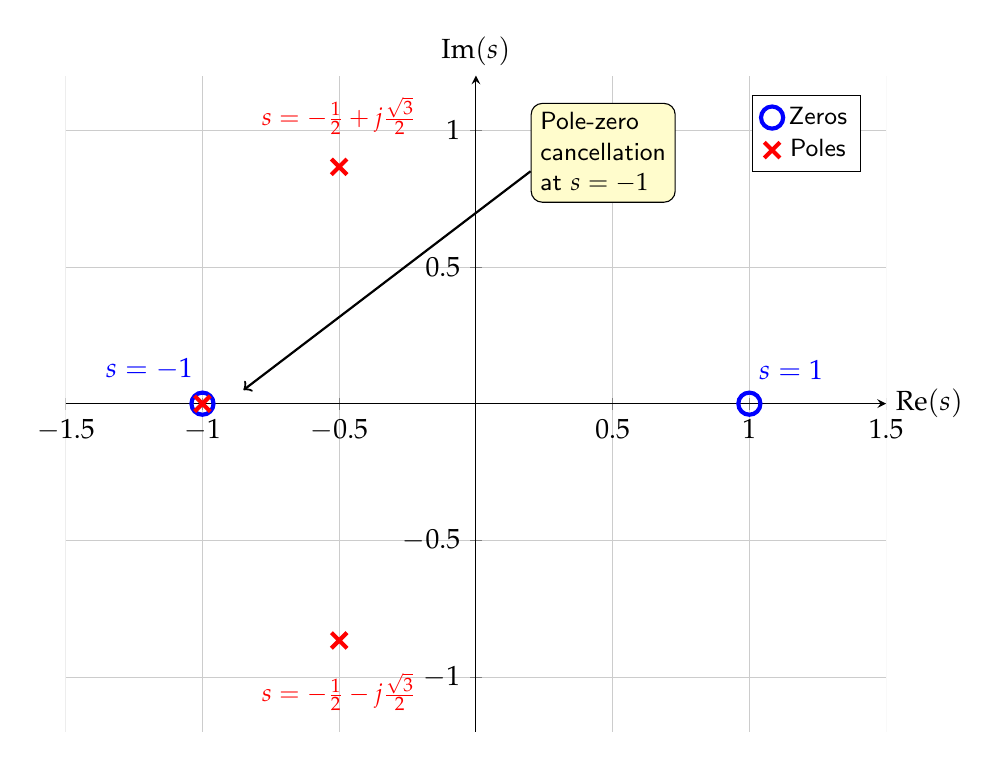
\begin{tikzpicture}
    \begin{axis}[
        width=12cm,
        height=10cm,
        axis lines=middle,
        xlabel={$\mathrm{Re}(s)$},
        ylabel={$\mathrm{Im}(s)$},
        xlabel style={anchor=west},
        ylabel style={anchor=south},
        xmin=-1.5, xmax=1.5,
        ymin=-1.2, ymax=1.2,
        xtick={-1.5,-1,-0.5,0,0.5,1,1.5},
        ytick={-1,-0.5,0,0.5,1},
        grid=both,
        grid style={line width=.1pt, draw=gray!20},
        major grid style={line width=.2pt,draw=gray!40},
        axis equal image,
        legend pos=north east,
        legend style={draw=black, fill=white, font=\small}
    ]
    
    % Zeros (circles)
    \addplot[only marks, mark=o, mark size=4pt, line width=1.5pt, color=blue] 
        coordinates {(1,0) (-1,0)};
    \addlegendentry{Zeros}
    
    % Poles (crosses) - complex conjugate pair
    \addplot[only marks, mark=x, mark size=4pt, line width=1.5pt, color=red] 
        coordinates {(-0.5,0.866) (-0.5,-0.866)};
    \addlegendentry{Poles}
    
    % Pole at s = -1 (this cancels with zero at s = -1)
    \addplot[only marks, mark=x, mark size=4pt, line width=1.5pt, color=red] 
        coordinates {(-1,0)};
    
    % Annotations
    \node[anchor=south west, color=blue] at (axis cs:1,0.05) {$s=1$};
    \node[anchor=south east, color=blue] at (axis cs:-1,0.05) {$s=-1$};
    \node[anchor=south, color=red, font=\small] at (axis cs:-0.5,0.95) {$s=-\frac{1}{2}+j\frac{\sqrt{3}}{2}$};
    \node[anchor=north, color=red, font=\small] at (axis cs:-0.5,-0.95) {$s=-\frac{1}{2}-j\frac{\sqrt{3}}{2}$};
    
    % Note about cancellation
    \node[anchor=north west, font=\small, align=left, fill=yellow!20, draw=black, rounded corners] 
        at (axis cs:0.2,1.1) {Pole-zero\\cancellation\\at $s=-1$};
    \draw[->, thick] (axis cs:0.2,0.85) -- (axis cs:-0.85,0.05);
    
    \end{axis}
\end{tikzpicture}
    
    \item After pole-zero cancellation:
    \[ H(s) = \frac{s - 1}{s^2 + s + 1} \]
    Poles: $s = -\frac{1}{2} \pm j\frac{\sqrt{3}}{2}$ \\
    Possible ROCs:
    \begin{itemize}
        \item $\text{Re}\{s\} > -\frac{1}{2}$: Causal
        \item $\text{Re}\{s\} < -\frac{1}{2}$: Anti-causal
    \end{itemize}
    
    \item Stability and causality:
    \begin{itemize}
        \item $\text{Re}\{s\} > -\frac{1}{2}$: Causal and stable (ROC includes $j\Omega$-axis)
        \item $\text{Re}\{s\} < -\frac{1}{2}$: Anti-causal and unstable
    \end{itemize}
    
    \item Impulse response for causal case:
    \begin{align*}
        H(s) &= \frac{s - 1}{s^2 + s + 1} = \frac{s - 1}{(s + \frac{1}{2})^2 + (\frac{\sqrt{3}}{2})^2} \\
        &= \frac{s + \frac{1}{2}}{(s + \frac{1}{2})^2 + (\frac{\sqrt{3}}{2})^2} - \frac{3}{2} \cdot \frac{1}{(s + \frac{1}{2})^2 + (\frac{\sqrt{3}}{2})^2} \\
        &= \frac{s + \frac{1}{2}}{(s + \frac{1}{2})^2 + (\frac{\sqrt{3}}{2})^2} - \sqrt{3} \cdot \frac{\frac{\sqrt{3}}{2}}{(s + \frac{1}{2})^2 + (\frac{\sqrt{3}}{2})^2}
    \end{align*}
    Taking inverse Laplace transform:
    \[ h(t) = \left[e^{-t/2}\cos(\frac{\sqrt{3}}{2}t) - \sqrt{3}e^{-t/2}\sin(\frac{\sqrt{3}}{2}t)\right]u(t) \]
\end{enumerate}

\section{Mixed Causal and Anti-Causal System}
Given the Laplace transform:
\[ X(s) = \frac{1}{s^2 - 4} \]
\begin{enumerate}[label=(\alph*)]
    \item Find all possible inverse Laplace transforms by considering different ROCs
    \item For each case, determine if the signal is causal, anti-causal, or two-sided
    \item For each case, determine if the signal is absolutely integrable (BIBO stable)
    \item Find the differential equation that has this as its characteristic equation
\end{enumerate}

\textbf{Solution:}
\begin{enumerate}[label=(\alph*)]
    \item Partial fraction expansion:
    \begin{align*}
        X(s) &= \frac{1}{s^2 - 4} = \frac{1}{(s - 2)(s + 2)} = \frac{A}{s - 2} + \frac{B}{s + 2} \\
        A & = \frac{1}{4}, \quad B = -\frac{1}{4} \quad \text{Using Partial Fraction}
    \end{align*}
    Therefore:
    \[ X(s) = \frac{1}{4} \cdot \frac{1}{s - 2} - \frac{1}{4} \cdot \frac{1}{s + 2} \]
    Possible ROCs and corresponding signals:
    \begin{itemize}
        \item $\text{Re}\{s\} > 2$: $x(t) = \frac{1}{4}[e^{2t} - e^{-2t}]u(t)$ (right-sided)
        \item $-2 < \text{Re}\{s\} < 2$: $x(t) = \frac{1}{4}[-e^{2t}u(-t) - e^{-2t}u(t)]$ (two-sided)
        \item $\text{Re}\{s\} < -2$: $x(t) = \frac{1}{4}[-e^{2t} + e^{-2t}]u(-t)$ (left-sided)
    \end{itemize}
    
    \item Signal properties:
    \begin{itemize}
        \item $\text{Re}\{s\} > 2$: Causal
        \item $-2 < \text{Re}\{s\} < 2$: Two-sided
        \item $\text{Re}\{s\} < -2$: Anti-causal
    \end{itemize}
    
    \item Absolute integrability (BIBO stability):
    \begin{itemize}
        \item $\text{Re}\{s\} > 2$: $e^{2t}$ grows without bound $\Rightarrow$ unstable
        \item $-2 < \text{Re}\{s\} < 2$: $e^{2t}$ term grows for $t < 0$ $\Rightarrow$ unstable
        \item $\text{Re}\{s\} < -2$: $e^{-2t}$ grows for $t < 0$ $\Rightarrow$ unstable
    \end{itemize}
    All cases are unstable.
    
    \item Differential equation:
    \begin{align*}
        X(s) &= \frac{1}{s^2 - 4} = \frac{Y(s)}{X(s)} \\
        s^2Y(s) - 4Y(s) &= X(s) \\
        \frac{d^2y(t)}{dt^2} - 4y(t) &= x(t)
    \end{align*}
\end{enumerate}

\section{System Interconnections}
Two systems are connected in cascade:
\begin{itemize}
    \item System 1: $H_1(s) = \frac{s}{s + 1}$ with ROC: $\text{Re}\{s\} > -1$
    \item System 2: $H_2(s) = \frac{1}{s + 2}$ with ROC: $\text{Re}\{s\} > -2$
\end{itemize}
\begin{enumerate}[label=(\alph*)]
    \item Find the overall transfer function $H(s) = H_1(s)H_2(s)$
    \item Determine the ROC of the overall system
    \item Find the impulse response of the overall system
    \item Is the overall system stable?
    \item What would be the ROC if the systems were connected in parallel?
\end{enumerate}

\textbf{Solution:}
\begin{enumerate}[label=(\alph*)]
    \item Overall transfer function:
    \begin{align*}
        H(s) &= H_1(s)H_2(s) = \frac{s}{s + 1} \cdot \frac{1}{s + 2} = \frac{s}{(s + 1)(s + 2)}
    \end{align*}
    
    \item ROC of cascaded system: Intersection of individual ROCs
    \begin{align*}
        \text{ROC}_1: & \quad \text{Re}\{s\} > -1 \\
        \text{ROC}_2: & \quad \text{Re}\{s\} > -2 \\
        \text{Overall ROC}: & \quad \text{Re}\{s\} > -1
    \end{align*}
    
    \item Impulse response using partial fractions:
    \begin{align*}
        H(s) &= \frac{s}{(s + 1)(s + 2)} = \frac{A}{s + 1} + \frac{B}{s + 2} \\
        A & = -1 \quad \text{Using Partial Fraction} \\
        B & = 2 \\
        H(s) &= -\frac{1}{s + 1} + \frac{2}{s + 2}, \quad \text{ROC: } \text{Re}\{s\} > -1 \\
        h(t) &= [-e^{-t} + 2e^{-2t}]u(t)
    \end{align*}
    
    \item The overall system is stable because the ROC ($\text{Re}\{s\} > -1$) includes the $j\Omega$-axis, and all poles ($s = -1, -2$) are in the LHP.
    
    \item For parallel connection:
    \begin{align*}
        H(s) &= H_1(s) + H_2(s) = \frac{s}{s + 1} + \frac{1}{s + 2} \\
        &= \frac{s(s + 2) + (s + 1)}{(s + 1)(s + 2)} = \frac{s^2 + 2s + s + 1}{(s + 1)(s + 2)} = \frac{s^2 + 3s + 1}{(s + 1)(s + 2)}
    \end{align*}
    ROC would still be the intersection: $\text{Re}\{s\} > -1$
\end{enumerate}

\section{Final Value Theorem Application}
A system has transfer function:
\[ H(s) = \frac{2}{s(s + 3)} \]
\begin{enumerate}[label=(\alph*)]
    \item Find the step response $y(t)$
    \item Use the final value theorem to find $\lim_{t\to\infty} y(t)$
    \item Verify your result by taking the limit of $y(t)$ as $t\to\infty$
    \item Under what conditions is the final value theorem valid?
\end{enumerate}

\textbf{Solution:}
\begin{enumerate}[label=(\alph*)]
    \item Step response:
    \begin{align*}
        Y(s) &= H(s)X(s) = \frac{2}{s(s + 3)} \cdot \frac{1}{s} = \frac{2}{s^2(s + 3)} \\
        &= \frac{A}{s} + \frac{B}{s^2} + \frac{C}{s + 3}
    \end{align*}
    Using partial fraction
    \begin{align*}
        A & = -\frac{2}{9}\\
        B & = \frac{2}{3}\\
        C & = \frac{2}{9}
    \end{align*}
    Therefore:
    \begin{align*}
        Y(s) &= -\frac{2}{9} \cdot \frac{1}{s} + \frac{2}{3} \cdot \frac{1}{s^2} + \frac{2}{9} \cdot \frac{1}{s + 3} \\
        y(t) &= \left[-\frac{2}{9} + \frac{2}{3}t + \frac{2}{9}e^{-3t}\right]u(t)
    \end{align*}
    
    \item Final value theorem:
    \begin{align*}
        \lim_{t\to\infty} y(t) &= \lim_{s\to 0} sY(s) = \lim_{s\to 0} s \cdot \frac{2}{s^2(s + 3)} \\
        &= \lim_{s\to 0} \frac{2}{s(s + 3)} = \infty
    \end{align*}
    
    \item Verification:
    \[ \lim_{t\to\infty} y(t) = \lim_{t\to\infty} \left[-\frac{2}{9} + \frac{2}{3}t + \frac{2}{9}e^{-3t}\right] = \infty \]
    
    \item The final value theorem is valid only if all poles of $sY(s)$ are in the left half-plane. Here, $sY(s) = \frac{2}{s(s + 3)}$ has a pole at $s = 0$ (on the imaginary axis), so the theorem gives an incorrect finite value. The actual response goes to infinity due to the double pole at the origin.
\end{enumerate}

\section{Relationship Between Differential Equation and Transfer Function}
A system is described by the differential equation:
\[ \frac{d^3y(t)}{dt^3} + 6\frac{d^2y(t)}{dt^2} + 11\frac{dy(t)}{dt} + 6y(t) = 2\frac{dx(t)}{dt} + x(t) \]
\begin{enumerate}[label=(\alph*)]
    \item Find the transfer function $H(s)$
    \item Find the poles and zeros
    \item Determine the impulse response for the causal system
    \item Find the response to $x(t) = e^{-t}u(t)$ with zero initial conditions
    \item Is the system stable?
\end{enumerate}

\textbf{Solution:}
\begin{enumerate}[label=(\alph*)]
    \item Taking Laplace transform (zero initial conditions):
    \begin{align*}
        (s^3 + 6s^2 + 11s + 6)Y(s) &= (2s + 1)X(s) \\
        H(s) &= \frac{Y(s)}{X(s)} = \frac{2s + 1}{s^3 + 6s^2 + 11s + 6}
    \end{align*}
    
    \item Factor denominator: $s^3 + 6s^2 + 11s + 6 = (s + 1)(s + 2)(s + 3)$ \\
    Zeros: $2s + 1 = 0 \Rightarrow s = -\frac{1}{2}$ \\
    Poles: $s = -1, -2, -3$
    
    \item Partial fraction expansion:
    \begin{align*}
        H(s) &= \frac{2s + 1}{(s + 1)(s + 2)(s + 3)} = \frac{A}{s + 1} + \frac{B}{s + 2} + \frac{C}{s + 3} \\
        A & = -\frac{1}{2} \\
        B &  = 3 \\
        C &= -\frac{5}{2}
    \end{align*}
    Therefore:
    \begin{align*}
        H(s) &= -\frac{1}{2} \cdot \frac{1}{s + 1} + 3 \cdot \frac{1}{s + 2} - \frac{5}{2} \cdot \frac{1}{s + 3}, \quad \text{ROC: } \text{Re}\{s\} > -1 \\
        h(t) &= \left[-\frac{1}{2}e^{-t} + 3e^{-2t} - \frac{5}{2}e^{-3t}\right]u(t)
    \end{align*}
    
    \item Response to $x(t) = e^{-t}u(t)$:
    \begin{align*}
        X(s) &= \frac{1}{s + 1} \\
        Y(s) &= H(s)X(s) = \frac{2s + 1}{(s + 1)^2(s + 2)(s + 3)}
    \end{align*}
    This requires partial fraction expansion with repeated poles. The solution would be similar to previous problems but more complex.
    
    \item The system is stable because all poles ($s = -1, -2, -3$) are in the LHP and the ROC for the causal system ($\text{Re}\{s\} > -1$) includes the $j\Omega$-axis.
\end{enumerate}


\end{document}